% ================================================
% =                 OBJECTIVES                   =
% ================================================ 
This master's thesis aims to address key challenges in \aclink{BEV} semantic segmentation. While initially motivated by the investigation of optimal BEV segmentation strategies, this work also explores a tangible real-world application of these techniques in the \aclink{ADS} context. Accordingly, it focuses on achieving two main objectives: to analyze semantic segmentation in \aclink{BEV} space for planar elements by comparing a traditional strategy with a proposed alternative approach (\textbf{O1}), and to implement an annotation system for generating BEV masks for occupancy, occlusion, and drivable areas (\textbf{O2}).

\begin{figure}[h!]
    \centering
    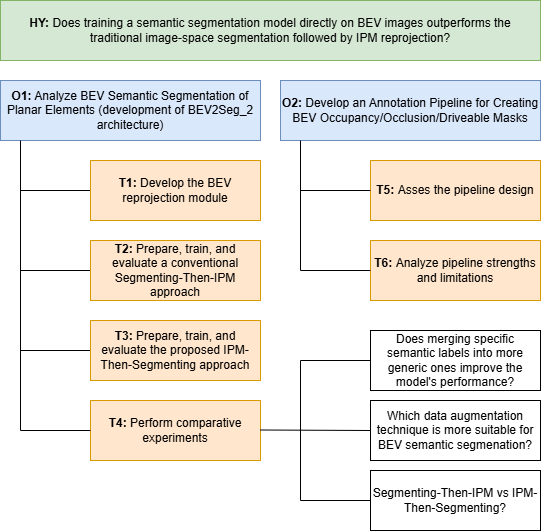
\includegraphics[width=0.8\linewidth]{./images/objectives/TFM_Objectives.png}
    \caption{Thesis objectives and tasks}
    \label{fig:objectives}
\end{figure}

To address the first objective, a methodology named BEV2Seg\_2 has been developed, establishing a common comparison framework between the classical image-space segmentation followed by \aclink{IPM} reprojection and the proposed direct \aclink{BEV} segmentation approach. Within this framework, a shared semantic segmentation model must be selected and adapted to both strategies to ensure consistency in the architecture design. The model will be trained under two different configurations: using conventional perspective images (\textbf{T2}), and using \aclink{BEV} reprojected images (\textbf{T3}). This dual training approach will produce two versions of the model architecture, each corresponding to one of the compared strategies.

To ensure a fair and valid comparison, the same original dataset will be used as the input source for both training pipelines. From this dataset, \aclink{BEV} reprojected images and their corresponding semantic masks will be generated to serve as training data for the proposed \aclink{BEV} based approach. Consequently, a common \aclink{BEV} reprojection module must be developed (\textbf{T1}). This module will apply consistent transformation parameters and serve two key purposes: generating the \aclink{BEV} training dataset and reprojecting inferenced results from the traditional strategy. In doing so, it ensures that both models are evaluated on an identical validation set composed of \aclink{BEV} semantic masks, thereby allowing for a reliable and unbiased performance comparison.

The second objective of this thesis involves developing a practical application of \aclink{BEV} semantic segmentation by implementing an automated annotation pipeline (\textbf{T5}). This pipeline aims to generate masks in \aclink{BEV} space that represent occupancy, occlusion, and drivable areas from vehicular scene data. This directly addresses the need for real-world utility of \aclink{BEV} semantic masks for downstream tasks such as motion planning and dynamic obstacle handling. Alongside the implementation, a critical analysis of the solution will be carried out to assess its effectiveness, strengths, and limitations (\textbf{T6}).

To achieve the stated objectives, this master's thesis relied on a diverse set of software tools and hardware resources for dataset generation, model training and validation, and annotation pipeline implementation. Python was the main programming language used for most of the custom implementations. Docker was extensively used for software packaging and environment consistency, facilitating interactions with a High-Performance Computing system for model training and enabling the creation of automated systems essential for annotation generation. Furthermore, various visualization tools such as WebLABEL and Open3D were employed to support development and analysis throughout the project.

This project was conducted over a seven-month period at Vicomtech  \footnote{\url{https://www.vicomtech.org/en/}}. Vicomtech, is a research center in applied Artificial Intelligence, VisualComputing, and Interaction which provided the necessary hardware infrastructure and technical support for this thesis.



% De esta manera, este trabajo busca cumplir con dos objetivos principales: analizar la segmentación semática en BEV para elementos planares de una estragia tradicional frente a la estrategia propuesta y realizar una implementación práctica de un sistema de pre-anotacion para crear máscaras BEV de ocupación/oclusion/area conducible. Para conseguir el primer objetivo, se ha desarrollado una metodología nombrada BEV2Seg_2 en la cual se establece un marco de comparación común para el approach clásico y el propuesto. En este marco de trabajo será necesario realizar la selección de un modelo de segmentación semántica que sea utilizado por las dos estrategias mencionadas. Este modelo será entrenado de formas distintas, con el fin de obtener las dos arquitecturas mencionadas: en la primera se utilizarán imágenes en perspectiva, y para la segunda imágenes en BEV. Para realizar estos entrenamientos asegurando una comparación justa entre las estrategias, es necesario que el dataset de partida original sea el mismo, generando a partir de las imágenes del dataset originales, las imágenes y máscaras reproyectadas en BEV para entrenar el approach propuesto. Es por ello, que se tiene que desarrollar un módulo de reporyección a BEV común que emplee los mismos parámetros y que se utilizará tanto para la generación del dataset de entrenamiento como para realizar las predicciones en tiempo de inferencia. De esta manera, también se asegurará que el conjunto de validación, compuesto por máscaras semánticas en BEV, de las dos estrategias es el mismo y se realiza una comparación justa. En cuanto al segundo objetivo, se busca implementar a practical application of \aclink{BEV} semantic segmentation by creating an automated pipeline for generating occupancy, occlusion, and drivable area masks from vehicular scenes. This directly addresses the need for real-world utility of \aclink{BEV} semantic masks for downstream tasks such as motion planning and dynamic obstacle handling. Todo esto junto con el análisis de la solución implementada








% ================================================ 
% This master's thesis aims to address key challenges in \aclink{BEV} semantic segmentation and its practical applications within autonomous driving systems. While initially motivated by the investigation of optimal BEV segmentation strategies, this work also explores a tangible real-world application of these techniques.
% Respectively, the main objectives of this thesis are:
% \begin{enumerate}
%     \item \textbf{Evaluate \aclink{BEV} segmentation strategies performance for planar elements:} To empirically determine whether a semantic segmentation model directly trained on \aclink{BEV} images outperforms a traditional pipeline that involves segmentation in image space followed by \aclink{IPM} reprojection, specifically focusing on the segmentation of planar elements. In addressing this primary question, other crucial sub-questions are also investigated:
%         \begin{itemize}
%             \item \textbf{Asses label merging impact:} To evaluate if merging semantically similar labels during training can enhance model performance, parcularly for low-presence classes in \aclink{BEV} images.
%             \item \textbf{Identify effective data augmentation:} To determine which data augmentation techniques are most effective for training semantic segmentation models directly on \aclink{BEV} images.
%         \end{itemize}
%     \item \textbf{Develop a \aclink{BEV} scene annotation pipeline:} To implement a practical application of \aclink{BEV} semantic segmentation by creating an automated pipeline for generating occupancy, occlusion, and drivable area masks from vehicular scenes. This directly addresses the need for real-world utility of \aclink{BEV} semantic masks for downstream tasks such as motion planning and dynamic obstacle handling.
% \end{enumerate}
% To achieve the stated objectives, this master's thesis relied on a diverse set of software tools and hardware resources for dataset generation, model training and validation, and annotation pipeline implementation. Python was the main programming language used for most of the custom implementations. Docker was extensively used for software packaging and environment consistency, facilitating interactions with a High-Performance Computing system for model training and enabling the creation of automated systems essential for annotation generation. Furthermore, various visualization tools such as WebLABEL and Open3D were employed to support development and analysis throughout the project.
% This project was conducted over a seven-month period at Vicomtech  \footnote{\url{https://www.vicomtech.org/en/}}. Vicomtech, is a research center in applied Artificial Intelligence, VisualComputing, and Interaction which provided the necessary hardware infrastructure and technical support for this thesis.
